%%%%%%%%%%%%%%%%%%%%%%%%%%%%%%%%%%%%%%%%%%%%%%%%%%%%%%%%%%%%%%%%%%% 
%                                                                 %
%                           INLEIDING                             %
%                                                                 %
%%%%%%%%%%%%%%%%%%%%%%%%%%%%%%%%%%%%%%%%%%%%%%%%%%%%%%%%%%%%%%%%%%% 


\chapter{Testen en Resultaten}  

In dit hoofdstuk worden de resultaten van het programma besproken. Vooraleer dit gedaan wordt zal er gekeken worden hoe de add-on moet worden geïnstalleerd en gebruikt. Dit zal worden gedaan aan de hand van een stappenplan.
\par
Er zal ook een vergelijking worden gedaan tussen een bestaand kristalvisualisatieprogramma en het programma als kristalvisualisatietool in Blender. Dit zal onder andere gedaan worden op basis van snelheid, gebruiksvriendelijkheid en uitbreidbaarheid.
\par
Er worden in dit hoofdstuk ook enkele valkuilen besproken die in de loop van dit onderzoek zijn opgedoken, en hoe deze worden opgelost. Sommige van deze valkuilen vormen echter grote problemen die in Blender moeilijk of niet kunnen worden vermeden. Er zal vermeld worden hoe deze problemen in dit onderzoek al dan niet zullen worden omzeild. Ten slotte zal er een blik worden geworpen op hoe het programma in de toekomst kan worden verbeterd en uitgebreid.
\par
Net zoals in hoofdstuk vier zal er voornamelijk gebruik worden gemaakt van de actieve schrijfwijze en de wetenschappelijke 'we'-vorm. 
\par 
In de eerste sectie staat een stappenplan dat het hele proces beschrijft dat moet gevolgd worden om met de add-on een kristal te tekenen in Blender. In de tweede sectie zullen resultaten van het programma worden beschreven. Hier worden onder andere enkele getekende kristallen weergegeven. In de derde sectie worden deze resultaten vergeleken met die van een ander kristalvisualisatieprogramma. 
\par
De vierde sectie zal de valkuilen bespreken waarmee dit onderzoek had te maken. In deze sectie worden ook enkele tekortkomingen van het programma gezien. In de vijfde, en voorlaatste, sectie van dit hoofdstuk wordt er gekeken naar wat de toekomst te bieden heeft voor het programma. Ten slotte zal er een conclusie gegeven worden waarin de belangrijkste punten van dit hoofdstuk nogmaals aan bod komen.   


\section{Een kristal tekenen met de add-on}
Deze sectie dient als een handleiding een gebruiker kan volgen om onze add-on te installeren in Blender en ze te gebruiken. Dit gaan we doen in de vorm van een stappenplan. 
\par
Dit is het stappenplan voor de installatie en het gebruik van de add-on op het besturingssysteem Windows. De add-on zou moeten werken op andere besturingssystemen maar de installatie van de add-on op deze gaan we niet bekijken. 

\subsection{Stap 1: Blender downloaden}
Als eerste moeten we Blender downloaden op ons syteem. Onze add-on is gemaakt voor versie 2.8x van Blender. In deze versie is er veel vernieuwd aan de Blender API waardoor de add-on niet achterwaarts compatibel is. Dit wil zeggen dat de add-on niet zal werken op oudere versies van Blender zonder de code aan te passen. In dit hoofdstuk spreken we, tenzij anders vermeld, altijd over de 2.8x versie van Blender .  
\par
Blender kan gedownload worden op de downloadpagina van hun offiële website:\url{https://builder.blender.org/download/}. Hier kiezen we het besturingssysteem en de bit-versie van ons systeem, en selecteren we de nieuwste versie van Blender, rode kader op Figuur[5.1].  Dit download het ZIP-bestand waarin de Blender installatie staat. Als de download voltooid is kunnen we het ZIP-bestand uitpakken op ons systeem. Dit creëert een map waarin de Blender installatie staat. In deze map vinden we het uitvoerbare bestand \textit{blender.exe}, waarmee we Blender opstarten. Dit is tevens ook de map waarin we de CifFile module in plaatsen, zie eerste sectie van hoofdstuk vier.      

\begin{figure}[h]
\begin{center}
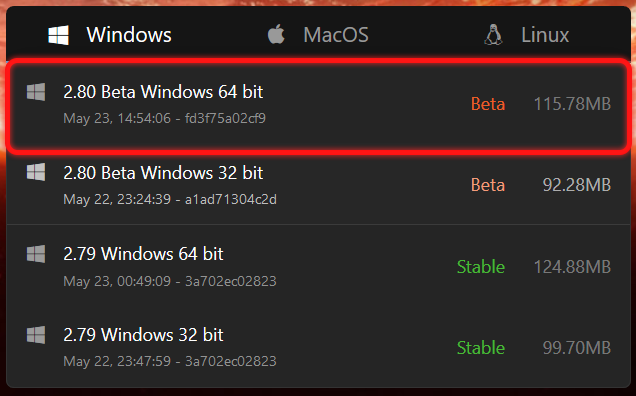
\includegraphics[scale=0.5]{b_download.png}
\caption{Overzicht van Blenderversies op downloadpagina van blender}
\end{center}
\end{figure}
 
\subsection{Stap 2: Externe programma's installeren}
Om de add-on te laten werken moeten we de OpenBabelGUI en de CifFile module van PyCIFRW op ons systeem installeren. We kunnen deze programma's downloaden op volgende webpagina's:

\begin{itemize}
\item OpenBabelGUI: \url{http://openbabel.org/wiki/Category:Installation}
\item PyCIFRW: \url{https://pypi.org/project/PyCifRW/#description}
\item CifFile module: \url{https://github.com/JarritB/Thesis/tree/master/} 
\end{itemize}   

Hoe we deze programma's werkende krijgen op ons systeem wordt uitgelegd in de eerste sectie van hoofdstuk vier. 
\par

\subsection{Stap 3: Add-on downloaden}
Een ZIP-bestand van de add-on kan worden gekopiëerd uit de bijlagen van deze tekst.[Bijlage G] De meest recente versie van de add-on vinden we op de GitHub pagina van dit onderzoek: \url{https://github.com/JarritB/Thesis/tree/master/blender-2.80.0-git.3c8c1841d72-windows64/2.80/scripts/addons} in de map \textit{crystallographic\_interface}. Deze map bevat de code en dictionaries van onze add-on.
\par  
We downloaden de map en plaatsen deze in de \textit{addons} submap van de Blender installatie. (\textit{blender-2.80.0-git.3c8c1841d72-windows64 \textgreater \textgreater{} 2.80 \textgreater \textgreater{} scripts\textgreater \textgreater{} addons}) 

\subsection{Stap 4: Add-on activeren}
Om de add-on te activeren moeten we eerste Blender opstarten door \textit{blender.exe} uit te voeren. Vervolgens gaan we het venster met de \textit{user preferences} openen. Dit kunnen we doen op twee manieren: 
\begin{itemize}
\item In de linkerbovenhoek bij de optie \textit{Edit} (links op Figuur[5.2])
\item Zoekfunctie openen (F3-toets), en \textit{Show User Preferences} intypen (rechts op Figuur[5.2]) 
\end{itemize}     

\begin{figure}[h]
\begin{center}
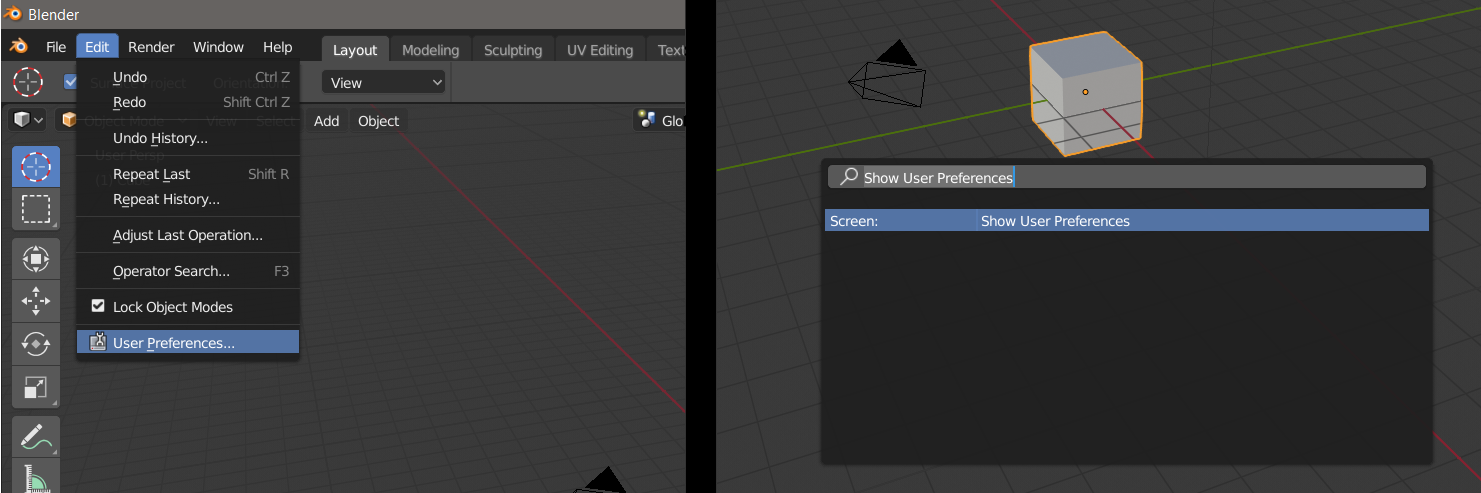
\includegraphics[width=\textwidth]{activ.png}
\caption{Openen van de \textit{User Preferences} via GUI(links) en Zoekfunctie(rechts)}
\end{center}
\end{figure}
 
Onder de tab \textit{add-ons} vinden we een lijst met add-ons die we kunnen gebruiken in Blender. Omdat we onze add-on in de map van Blender hebben geplaatst zou deze in de lijst moeten te vinden zijn onder de naam: \textit{Crystallography in Blender: Crystallographic Drawing Tool for Blender}. Om de add-on te activeren hoeven we enkel het selectievakje links van de naam aan te duiden. Als het vakje is aangevinkt is de add-on geactiveerd en klaar voor gebruik.

\subsection{Stap 5: Kristal tekenen met de add-on}
We kunnen de label van onze add-on zien onder het veld \textit{Tools} op het \textit{3D View} venster. Dit is het grote venster in het midden dat we zien wanneer we Blender opstarten. Het \textit{Tools} veld vinden we aan de linkerkant van dit venster, maar kan verborgen zijn. Met de T toets tonen en verbergen we tools veld. Bij het aanklikken van het \textit{CDTB} label zal ons paneel tevoorschijn komen. Als we osn in 'Edit Mode' bevinden zal het label niet getoont worden, door de Tab toets in te drukken geraken we terug in 'Object Mode', waar onze add-on zou moeten staan.  
\par   


Om een kristal te tekenen moeten we eerst een CIF-bestand selecteren. Dit doen we door met het icoon naast "Select a file" een bestandsbrowser te openen en ons CIF-bestand te selecteren. Dan hebben we de mogelijkheid om een aantal tekenvoorkeuren aan te passen, in Tabel[5.1] worden deze uitgelegd. Als we de voorkeuren hebben aangepast hoeven we enkel nog op de \textit{Draw Crystal} knop te klikken, en te wachten tot het kristal getekend is. Dit duurt, afhankelijk van de gekozen tekenopties en de grootte van het kristal, enkele seconden tot enkele minuten.
\par

\begin{table}[H]

\begin{center}
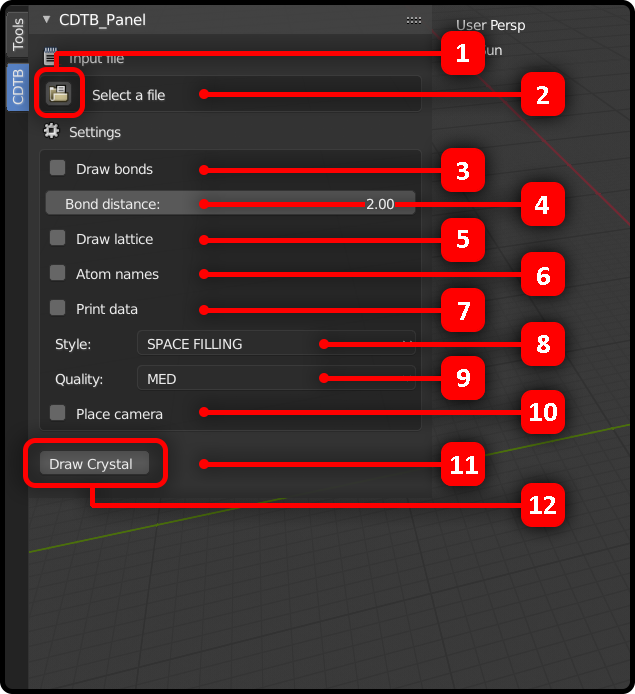
\includegraphics[scale=0.7]{numbers.png}
\end{center}

\begin{tabular}{|l|l|}
\hline
1  & Bij indrukken: opent een bestandsbrowser waar het CIF-bestand kan geselecteerd worden                                                                                                                                                                                \\ \hline
2  & Toont het geselecteerde CIF-bestand                                                                                                                                                                                                                                  \\ \hline
3  & Als aangeduid: tekent bindingen tussen de atomen                                                                                                                                                                                                                     \\ \hline
4  & Getal: bepaalt maximale afstand waartussen twee atomen worden gebonden                                                                                                                                                                                               \\ \hline
5  & Als aangeduid: tekent omkadering van de eenheidscel                                                                                                                                                                                                                  \\ \hline
6  & Als aangeduid: toont namen van de atomen op de tekening                                                                                                                                                                                                              \\ \hline
7  & Als aangeduid: drukt de kristalinformatie af in de Blender terminal                                                                                                                                                                                                  \\ \hline
8  & \begin{tabular}[c]{@{}l@{}}Keuzelijst: tekent kristal in gekozen stijl \\ \qquad STICK: toont enkel bindingen; \\ \qquad BALL AND STICK: toont verkleinde atomen, bindingen zichtbaar;\\ \qquad SPACE FILLING: toont atomen op ware grootte, bindingen meestan niet zichtbaar\end{tabular} \\ \hline
9  & Keuzelijst: bepaalt kwaliteit van de vormen, hogere kwaliteit verhoogt tekenduur                                                                                                                                                                                     \\ \hline
10 & Als aangeduid: plaats een camera en belichting, voor het renderen(F12) van het kristal                                                                                                                                                                               \\ \hline
11 & Bij indrukken: visualiseert het CIF-bestand                                                                                                                                                                                                                          \\ \hline
12 & Toont opmerkingen aan de gebruiker                                                                                                                                                                                                                                   \\ \hline
\end{tabular}
\caption{Overzicht van de instellingen van de add-on}
\end{table}
  
\section{Resultaten}

\subsection{Snelheid}

In een gebruiksvriendelijk programma speelt de snelheid ervan een belangrijke rol. We willen de tijd die een gebruiker moet wachten beperken, maar niet ten koste van van de kwaliteit van de uitvoer. In dit deel van de sectie gaan we kijken naar de duur van het programma bij verschillende parameters en welk deel van het programma het grootste aandeel van de tijd opeist. Merk op dat snelheid vaak evenredig is met de specificaties van het systeem. De specificaties van het systeem waarop we de testen gaan uitgevoeren zijn te vinden in de bijlages.[Bijlage H]  
\par
Eerst gaan we de totale duur van het programma testen bij het tekenen van kristallen. Deze testen worden gedaan voor drie kristallen met verschillende grootte. De resultaten van deze testen worden weergegeven op de grafieken in Figuur[5.3]. Enkele opmerkingen bij deze grafieken zijn:
\begin{itemize}
\item Op de verticale as wordt de loopduur in seconden weergegeven
\item Op de horizontale as worden wordt de tekenkwaliteit weergegeven
\item Het verhogen van de tekenkwaliteit gebeurt met factor vier per stap, en begint bij 32 segmenten
\item De tekenstijl \textit{LOW} hebben we niet getest
\item De getallen in de legende van de eerste grafiek zijn het aantal getekende atomen
\item De getallen in de legende van de tweede grafiek zijn het aantal getekende bindingen, het aantal atomen is gelijk aan de waarden in de eerste grafiek 
\item De gegeven waarden zijn telkens het gemiddelde van drie testen 
\item Deze resultaten zijn voor het tekenen van het "BALL AND STICK" model.
\item Hoewel de andere kristalvoorstellingen ook zijn getest, kregen we gelijkaardige waarden aan die van het "BALL AND STICK" model en worden deze niet gepubliceert.
\item Bij het testen werd enkel de kristalomkadering getekend, andere instellingen werden uitgezet 

\end{itemize}

\begin{figure}[H]
\begin{center}
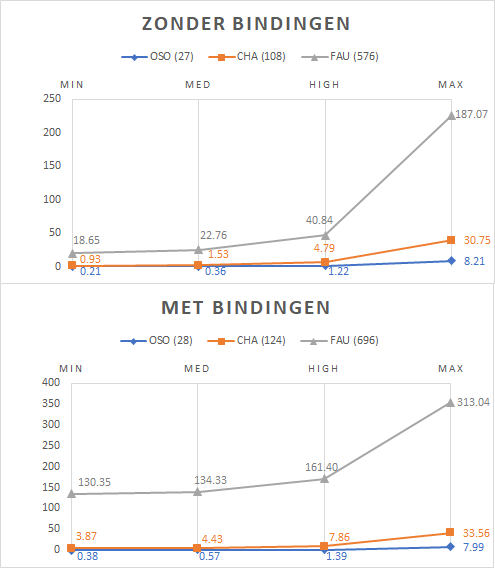
\includegraphics[width=\textwidth]{graphs_spd.png}
\caption{Duur van het programma in functie van gekozen kwaliteit}
\end{center}
\end{figure}

Aan de hand van deze resultaten kunnen we er vanuit gaan dat de duurtijd evenredig is met het aantal atomen dat moeten getekend worden. We merken op dat dit geen recht evenredig verband is, het kristal FAU bestaat uit ongeveer vijf keer meer atomen dan CHA, terwijl de tekenen van FAU een factor 20 langer duurt. Dit kan het gevolg zijn van het stelselmatig vol geraken van het werkgeheugen, wat kan leiden tot vertraging van het systeem.  
\par
Het aantal bindingen dat wordt getekend heeft ook een grote impact op de snelheid. We stellen vast dat het tekenen van de bindingen een vaste tijd duurt, ongeacht de tekenkwaliteit. Dit is omdat de tekenkwaliteit enkel invloed heeft op het aantal segmenten van de atomen. We kunnen dit grafisch waarnemen doordat de grafieken ruwweg dezelfde vorm tonen maar verschoven zijn naar boven. Door deze vaste duur zal het aandeel aan tijd dat het tekenen van de bindingen in beslag neemt groter zijn bij een lagere kwaliteit. Bij FAU zal het tekenen van de bindingen op de laagste tekenkwaliteit tot wel 85 procent van de totale loopduur van het programma opeisen, terwijl dit bij de hoogste kwaliteit nog maar 40 procent is.

\subsection{Output van het programma}
In dit deel kijken we voornamelijk naar hoe ons programma kristallen afbeeld in Blender. We gaan, met behulp van figuren, bekijken hoe de verschillende modellen eruitzien, hoe we door het verhogen van de kwaliteit een mooier beeld krijgen en wat er gebeurt als we ons kristal gaan renderen.
\par
Op figuur[5.4] kunnen we de invloed zien van de kwaliteit, e.i. het aantal segmenten, van de atomen. In de linkerkolom staan de tekeningen zoals ze in Blender worden weergegeven en in de rechterkolom vinden we de gerenderde tekeningen. We hebben bewust gekozen de stapgrootte tussen deze voorbeelden constant te houden. Tabel[5.2] toont het aantal segmenten per atoom voor de verschillende tekenkwaliteiten. Door de exponentiele toename zou het verschil tussen de kwaliteiten duidelijk zichtbaar moeten zijn. Dit is ook zo, tot op een bepaald punt. Er is een duidelijk verschil tussen de eerste en tweede afbeelding van de linkerkolom van Figuur[5.4], de twee onderste afbeeldingen zijn echter al moeilijker van elkaar te onderscheiden. En wetende dat er tussen deze twee nog een stap zit, kunnen we vaststellen dat het, in de meeste gevallen, niet noodzakelijk is in de hoogste kwaliteit te tekenen.   
\par
\begin{table}[H]
\begin{tabular}{|l|l|}
\hline
MIN  & 32   \\ \hline
LOW  & 128  \\ \hline
MED  & 512  \\ \hline
HIGH & 2048 \\ \hline
MAX  & 8192 \\ \hline
\end{tabular}
\caption{Segmenten per atoom bij bepaalde kwaliteit}
\end{table}
\par
Een voorbeeld van zo een geval waarbij we de hoogste kwaliteit willen is wanneer we ons kristal willen renderen naar een afbeelding. Het concept renderen hebben we reeds besproken in de vijfde sectie van het tweede hoofdstuk. In de rechterkolom van Figuur[5.4] staan de gerenderde versies van de linkerkolom. Nu er belichting aan te pas komt wordt het verschil in kwaliteit tussen de onderste twee duidelijk. Dit is dan ook de voornaamste reden om in de hoogste kwaliteit te tekenen.   
\par


\begin{figure}[H]
\begin{center}
\begin{tabular}{l|l}

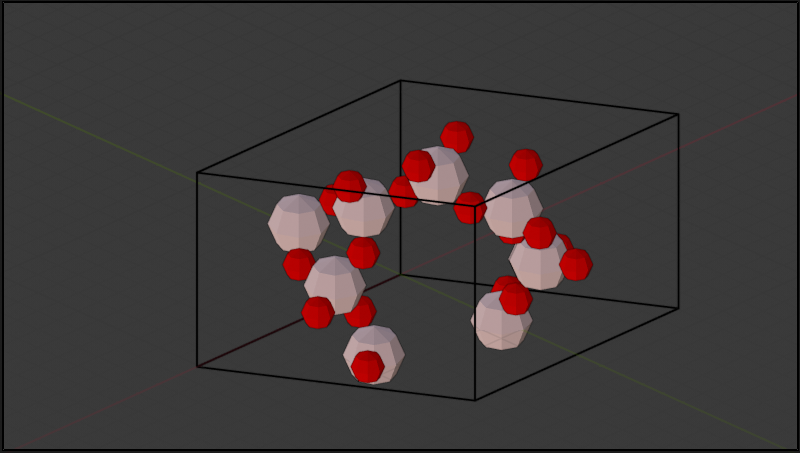
\includegraphics[width=\paperwidth/3]{OSO_min.png}
&
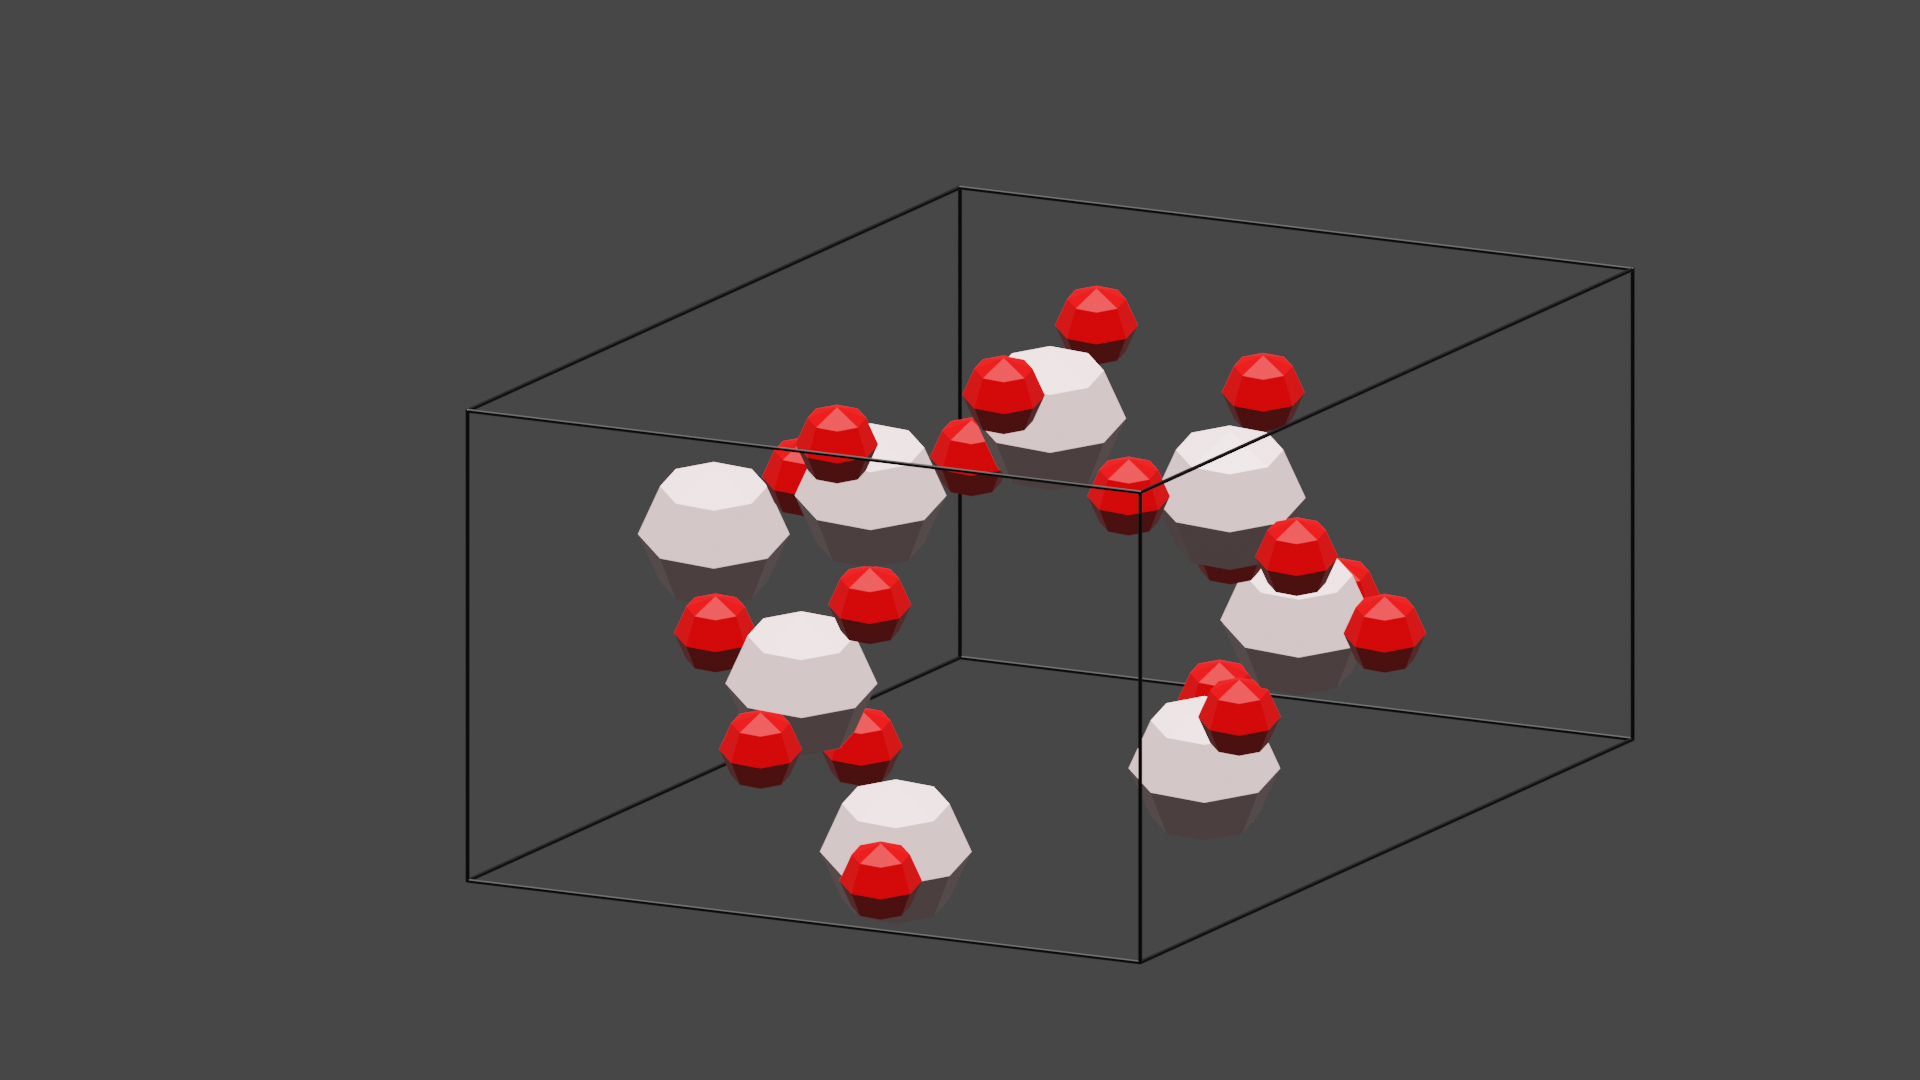
\includegraphics[width=\paperwidth/3]{OSO_minRen.png}
\\ 
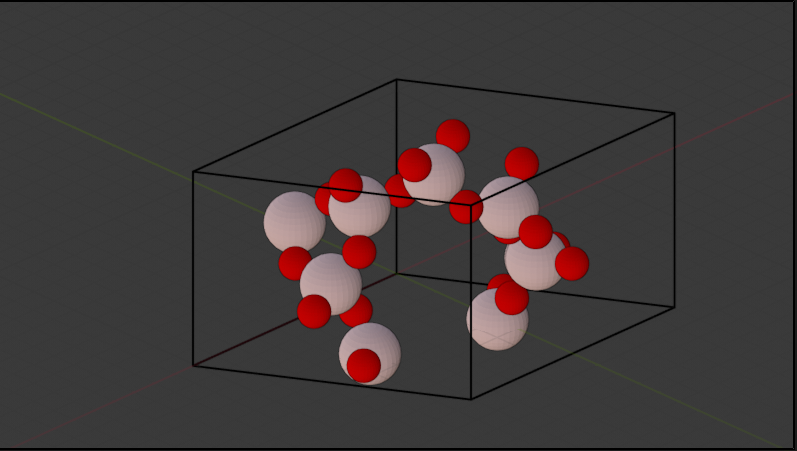
\includegraphics[width=\paperwidth/3]{OSO_med.png}
&
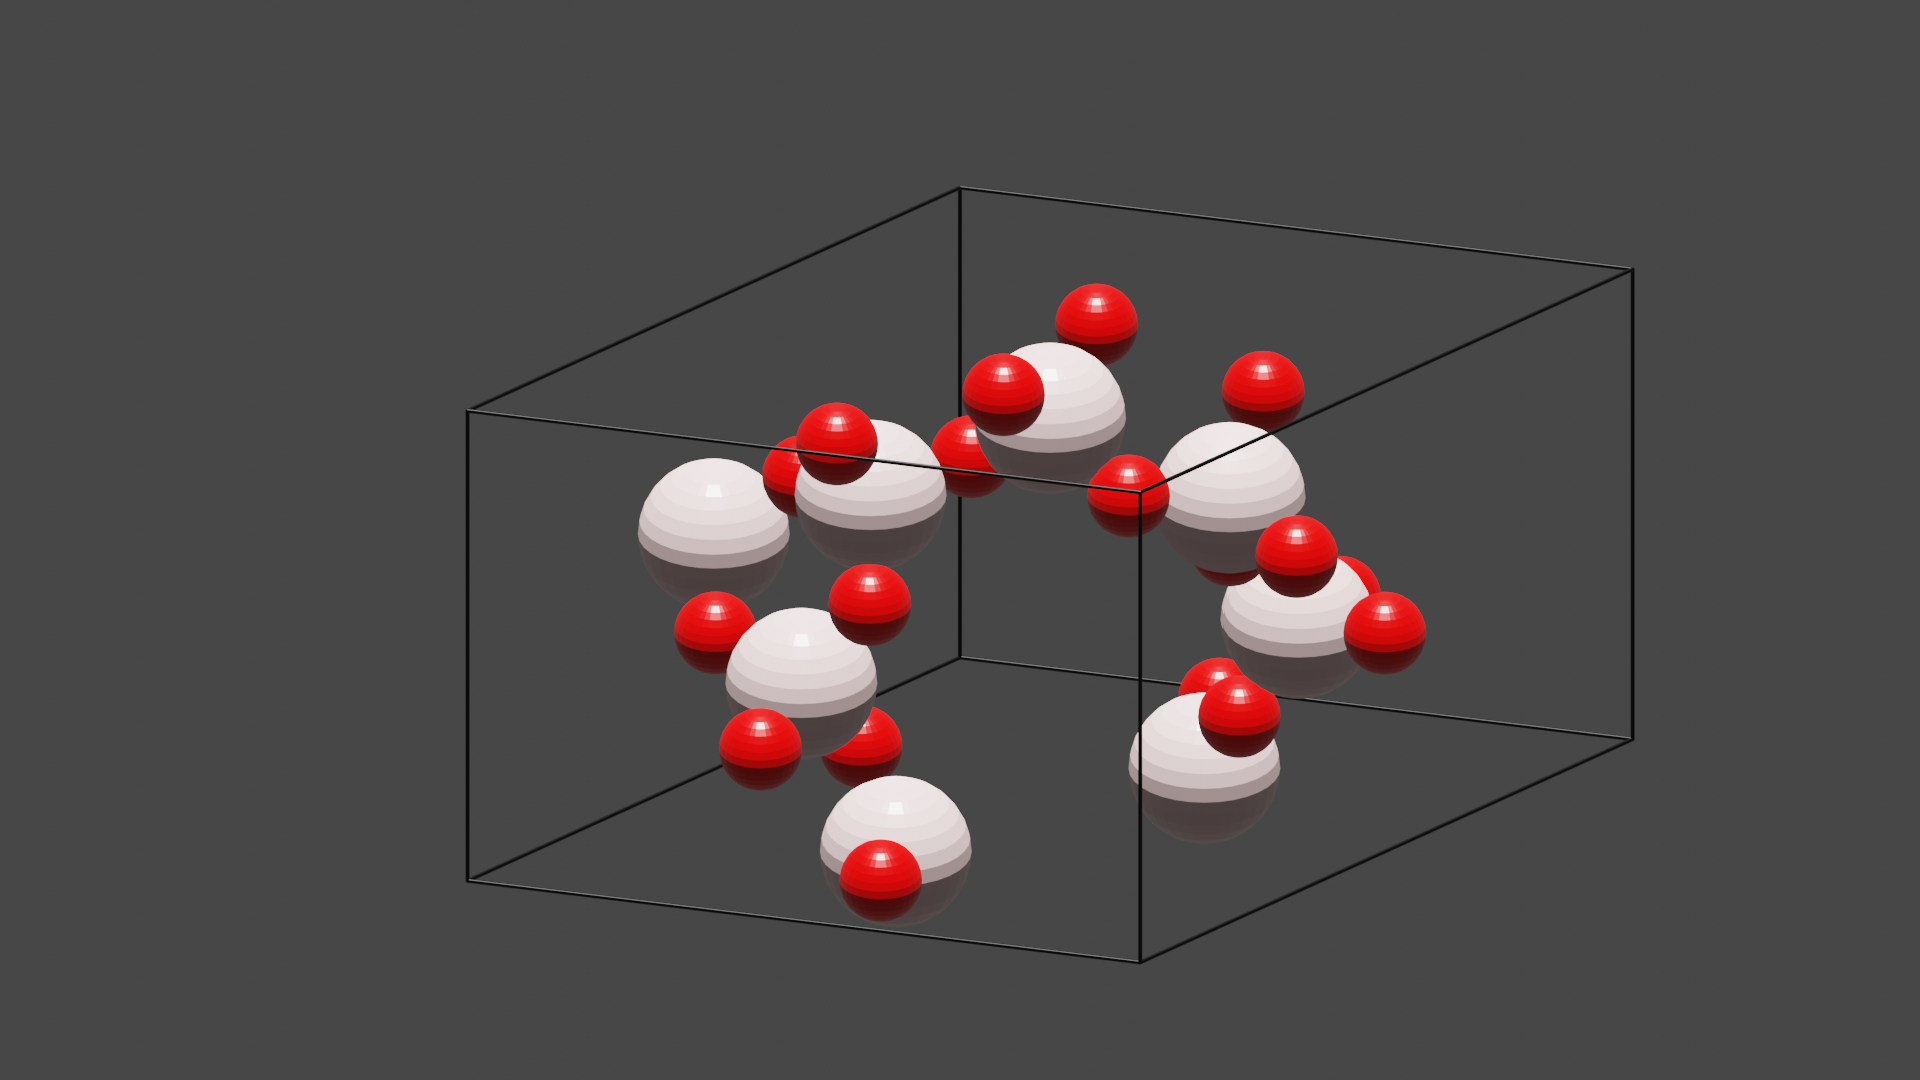
\includegraphics[width=\paperwidth/3]{OSO_medRen.png}
\\ 
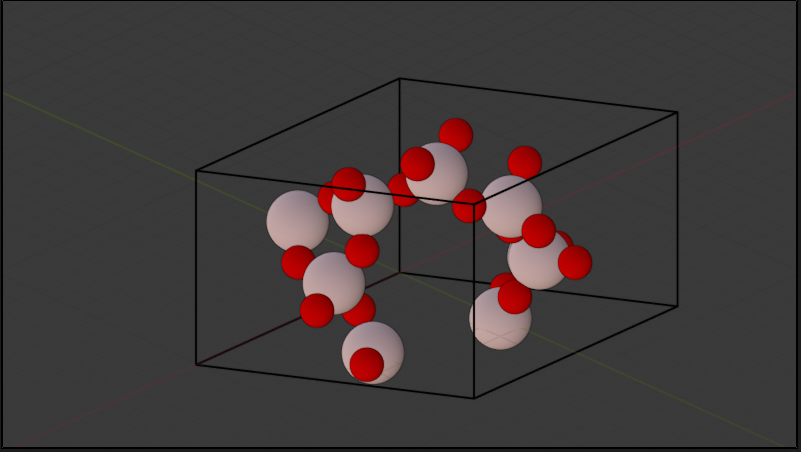
\includegraphics[width=\paperwidth/3]{OSO_max.png}
&
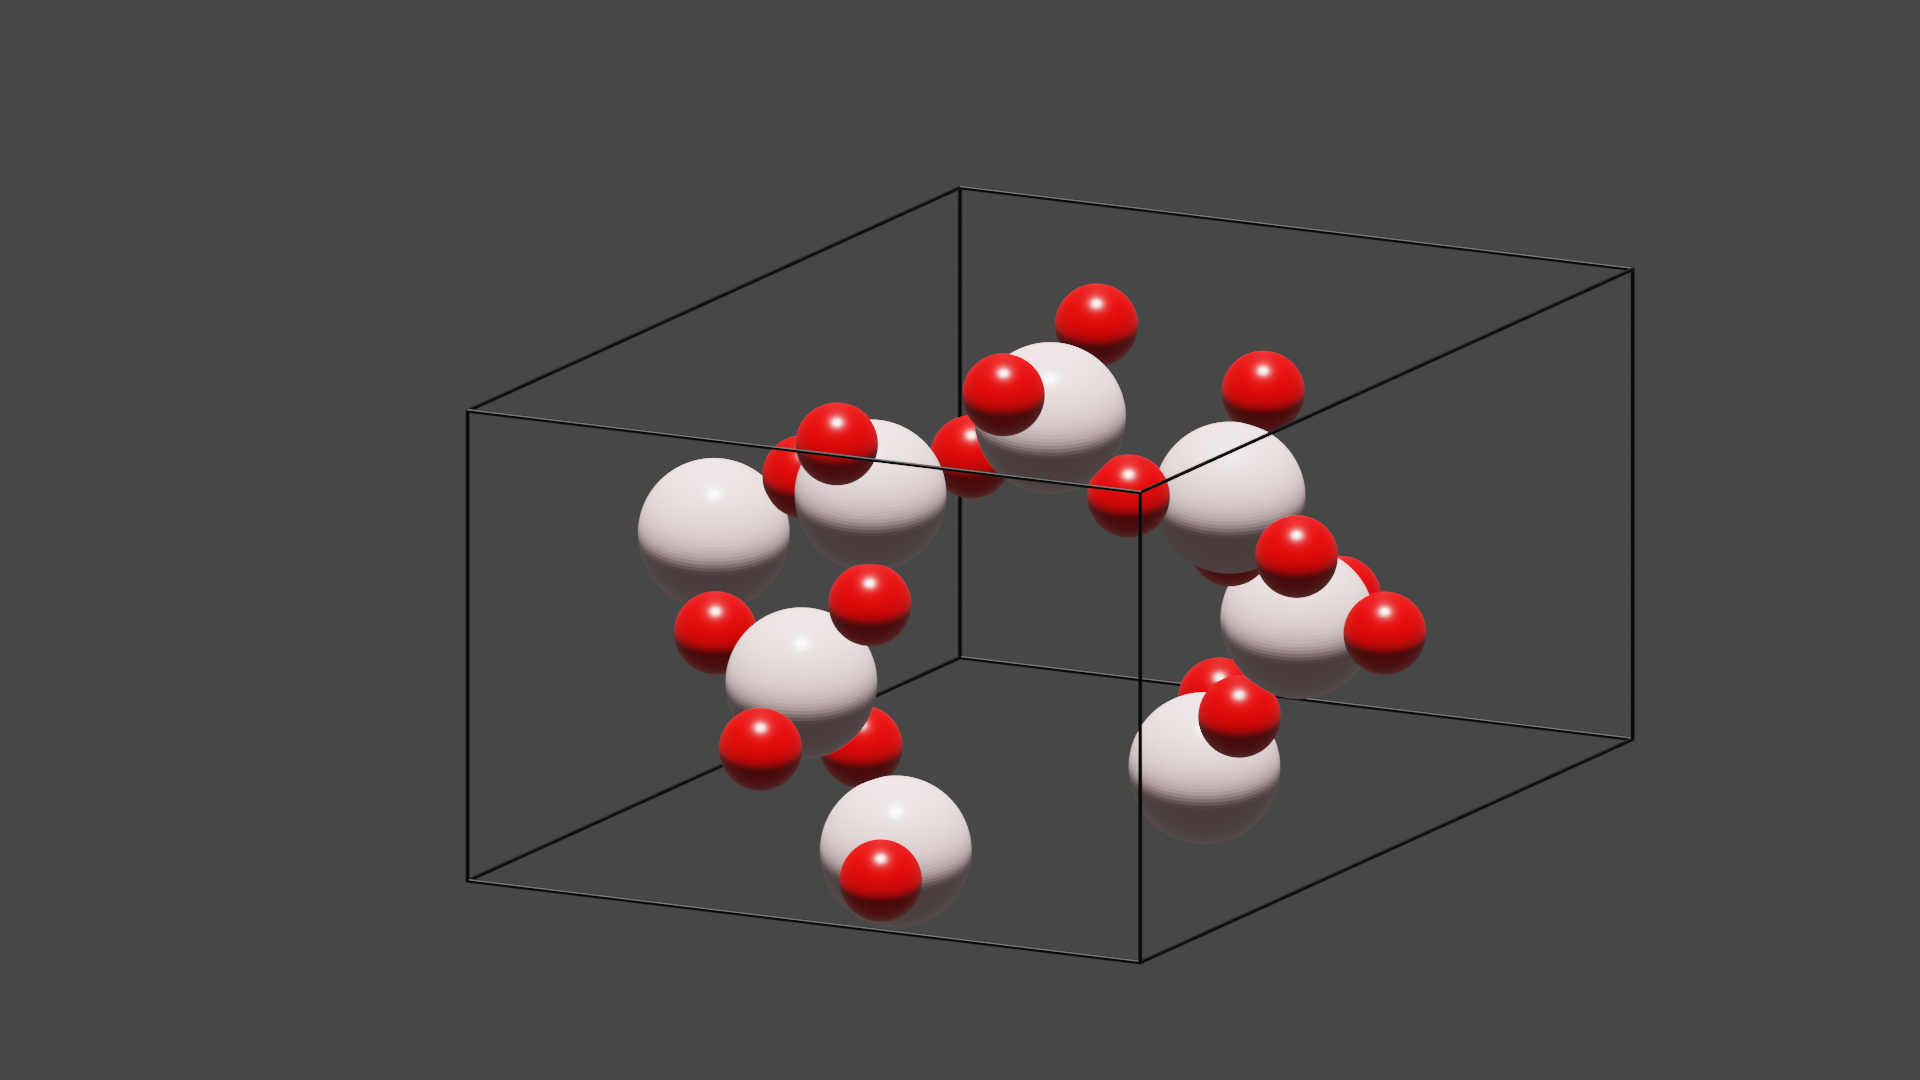
\includegraphics[width=\paperwidth/3]{OSO_maxRen.png}
\end{tabular}
\end{center}
\caption{Vergelijking van de tekenkwaliteit voor het kristal OSO (van boven naar onder: MIN MED MAX)}
\end{figure}



\section{Vergelijking met VESTA}  
Met deze resultaten kunnen we een vergelijking maken met een bestaand kristalvisualisatieprogramma. Als programma hebben we gekozen voor VESTA, omdat dit het meest gebruikte en meest performante is.

\subsection{Snelheid}
In Tabel[5.3] wordt de tekensnelheid van ons programma vergeleken met die van VESTA. Dit doen we voor de drie kristallen van Figuur[5.3]. In VESTA worden eerst de berekeningen gedaan van de posities van de atomen en bindingen, dan worden deze pas weergegeven. VESTA geeft echter enkel de tijd die nodig was om de berekeningen te maken. Doordat de kristallen vrijwel ogenblikkelijk verschijnen, is het erg moeilijk de werkelijke tekenduur te bepalen. Het is ook belangrijk op te merken dat VESTA meer atomen tekent per kristal, omdat het ook atomen buiten de eenheidscel tekent, terwijl ons programma enkel de atomen erbinnen tekent. Om de vergelijking eerlijk te maken zullen we in beide programma's de bindingen tussen de atomen tekenen. De duur wordt weergegeven in seconden en de kwaliteit staat in beide programma's op 512 segmenten  per atoom.
\par

\begin{table}[H]
\begin{center}
\begin{tabular}{|l|l|l|l|l|}
\hline
			              & Blender    	& VESTA & Factor \\ \hline
\multicolumn{1}{|l|}{OSO} & .570    	& 0.034 & 16.67  \\ \hline
\multicolumn{1}{|l|}{CHA} & 4.430   	& 0.062 & 71.45  \\ \hline
\multicolumn{1}{|l|}{FAU} & 134.330 	& 0.331 & 405.83 \\ \hline
\end{tabular}
\end{center}
\caption{Vergelijking in tekenduur tussen ons programma en VESTA, tijd in seconden}
\end{table}
In de laatste kolom wordt vermeld hoeveel maal sneller het tekenen in VESTA wordt gedaan ten op zichte van het tekenen in Blender. Het valt op dat VESTA kristallen veel sneller tekent, bij grote kristallen tot zelfs 400 maal sneller. Als we geen bindingen zouden tekenen met de add-on, zou deze factor nog 70 bedragen, wat een redelijke afname is, maar nog steeds een groot getal is. 
\par
Uit deze resultaten kunnen we concluderen dat het tekenen van kristallen met onze add-on veel langer duurt dan in VESTA, en het verschil in duur toeneemt bij het tekenen van grotere kristallen.  

\subsection{Gebruiksvriendelijkheid}	 
Ook op het vlak van gebruiksvriendelijkheid scoort VESTA erg hoog. VESTA is eenvoudig te downloaden, kristallen worden eenvoudig maar duidelijk weergegeven en kan naast het CIF-formaat ook andere formaten visualiseren. Er zijn een groot aantal tekenopties waarmee onder andere de tekenstijl, grenzen en kleuren kunnen worden aangepast. Hiernaast bezit VESTA een aantal handige features waarmee er specifieke informatie over het kristal kan worden berekend en weergegeven. Om deze features te gebruiken heeft de gebruiker wel een bepaalde kennis over het programma nodig. Een laatste en niet  onbelangrijke eigenschap van VESTA is dat het volledig gratis is.
\par
We hebben er naar gestreeft onze add-on zo gebruiksvriendelijk mogelijk te maken. Door het eenvoudig maar duidelijke paneel is onze add-on gemakkelijk in omgang, zelfs voor onervaren gebruikers. Het aantal features is eerder beperkt in vergelijking met VESTA. Zo is er, buiten de namen van atomen, geen mogelijkheid tot het weergeven van kristalinformatie en zijn de tekengrenzen beperkt tot binnen de eenheidscel. 
\par
Als we kijken naar de weergave van het kristal merken we dat het getekende kristal in Blender veel interactiever is dan in VESTA mogelijk is. In Blender kunnen we individuele atomen verplaatsen, verwijderen en verschalen. Terwijl VESTA deze mogelijkheid niet biedt.
\par
Met deze informatie is het moeilijker een winaar te kiezen op vlak van gebruiksvriendelijkheid dan het was bij de tekensnelheid van de programma's. Dit is deels omdat beide programma's hun voordelen en beperkingen hebben, en veel afhangt van het doel van de gebruiker. Voor een meer wetenschappelijke aanpak zullen we VESTA verkiezen, terwijl voor een meer interactieve oplossing onze add-on kan gebruikt worden.

\subsection{Uitbreidbaarheid}
Dit is het vlak waar onze add-on schitterd, en de voornaamste reden van dit onderzoek. 
\par
Hierboven hebben we VESTA geprezen voor het groot aantal features die het aanbiedt in vergelijking met onze add-on. Nu echter de basis van onze add-on is gelegd, kunnen we deze verder uitbreiden en allerlei features toevoegen. Het zelf creëren van features is met VESTA niet mogelijk. Hoewel VESTA enkele maal per jaar een update krijgt, zijn dit voornamelijk bugfixes en ligt het volledig in de hand van de makers of er nieuwe features worden toegevoegd.   
\par
Op vlak van uitbreidbaarheid is onze add-on de grote winnaar. Het toevoegen van features aan de add-on is een kwestie van functies code toe te voegen aan de broncode van het programma. In de vierde sectie van dit hoofdstuk gaan we in meer detail mogelijke uitbreidingen bespreken. 


\section{Valkuilen en problemen}

\subsection{Blender 2.80}
Zoals eerder gezegd werken we in dit onderzoek met Blender versie 2.80. Deze versie van Blender is op het moment van dit onderzoek nog in beta, dit wil zeggen dat Blender, hoewel bruikbaar, constant onder constructie is. Dit kan leiden tot instabiliteit van de software wat een risico vormde voor dit onderzoek. Ondanks het risico, zijn er in de loop van dit onderzoek geen problemen geweest als gevolg van deze instabiliteit.
\par
Doordat er in de 2.80 versie veel is veranderd ten op zichte van eerdere versies, en deze relatief nieuw is, was het geregeld moeilijk correcte informatie te vinden op fora. De Blender API heeft gelukkig een zeer duidelijke documentatie die vaak werd geraadpleegd in dit onderzoek.\citep*{BLEN3} 
\par


\subsection{PyCIFRW}
In de vierde sectie van het tweede hoofdstuk testen wordt er uitgelegd hoe we gaan controleren of de OpenBabel geïnstalleerd is op het systeem. In het geval dat deze installatie niet wordt gevonden staat er: "Hoewel het kristal niet kan geconverteerd worden, zullen we toch een deel van het kristal kunnen tekenen." Door een probleem in de CifFile module verschijnt er een foutboodschap als er een te lange padnaam wordt meegegeven bij het inlezen van het CIF-bestand. Doordat de bestandsbrowser steeds het volledige pad geeft kan dit probleem zeer moeilijk worden opgelost, en zelfs dan zouden enkel bestanden in de map van Blender kunnen ingelezen worden. 
\par
Zodra PyCIFRW een update krijgt, die dit probleem oplost, zou onze add-on moeten werken zelfs zonder installatie van OpenBabel. Tot dan zal het kristal niet kunnen getekend worden zonder OpenBabel.

\subsection{Bpy module}   
In de vorige hoofdstukken hebben we opgemerkt dat het tekenen van kristallen relatief lang duurt, zeker in vergelijking met VESTA. Dit ligt deels aan het feit dat de bpy module van Blender eerder traag is. Doordat we deze meerdere malen moeten oproepen telkens we een atoom of binding tekenen, duurt het lang voordat het volledige kristal getekend wordt.
\par
Dat tekenen met de bpy module eerder traag is kunnen we bewijzen aan de hand van een test. We schrijven een functie, Listing[5.1], die enkel bollen tekent en meten de tijd dat dit duurt. Door deze tijd te vergelijken met de tijd dat ons programma nodig heeft om een kristal zonder bindingen te tekenen weten we ruwweg hoelang ons programma bezig is met de berekeningen. De resultaten worden in Tabel[5.4] weergegeven. Bij de testen is het aantal segmenten per bol gebruikt dat overeenstemt met de \textit{MED} tekenkwaliteit.

\begin{lstlisting}[caption="Testprogramma dat een aantal bollen tekent en timed"]
import time
import bpy
S = time.time()
for i in range(576):
    bpy.ops.mesh.primitive_uv_sphere_add(segments=32,ring_count=16,size=0.5,location = (0,0,i))
    
print(time.time()-S)
\end{lstlisting}

\begin{table}[H]
\begin{center}
\begin{tabular}{|l|l|l|l|l|l|}
\hline
\# atomen & Programma 	& Testfunctie	& Verschil & \%	\\ \hline
27  & 0.36    & 0.29 		& 0.07  	&	19.4 \\ \hline
108 & 1.53   	& 1.31 		& 0.22  	&	14.3 \\ \hline
576 & 22.76 	& 16.95 	& 5.81 		&	25.5 \\ \hline
\end{tabular}
\end{center}
\caption{Vergelijking duur van ons programma en het tekenen van enkel bollen, tijd in seconden}
\end{table}

Uit Tabel[5.4] leiden we af dat ons programma gemiddeld 80 procent van de totale loopduur besteet aan het tekenen van de atomen. Hoewel dit kan gezien worden als een \textit{bottleneck} van het programma, kunnen we hier weinig of niets aan veranderen en zijn we beperkt de overige 20 procent te optimaliseren. 

\section{Uitbreidingen}
In deze sectie bespreken we enkele uitbreidingen die we in de toekomst nog kunnen worden uitgevoerd. Hoewel de lijst van mogelijke uitbreidingen op zich eindeloos is omdat met de combinatie van Python modules en de Blender API bijna alles mogelijk is, zullen we ons beperken tot de enkele belangrijke features.

\subsection{Bepalen van grenzen}
Eén feature dat voorlopig nog niet aanwezig is in de add-on, is de mogelijkheid tot het bepalen van de grenzen tot waar getekend moet worden. Deze grenzen zijn op dit moment de vlakken van het eenheidskristal. Door deze grenzen uit te breiden zal de gebruiker zelf kunnen kiezen hoe groot het getekende kristal mag zijn. 
\par
Om deze feature te verwezenlijken zullen we vanuit de inwendige symmetrie van het kristal een lijst moeten maken van alle atomen die binnen deze grenzen liggen. Aangezien OpenBabel deze mogelijkheid niet aanbiedt, zal er moeten gezocht worden naar een programma dat dit wel kan, of zullen we zelf een functie moeten schrijven die de plaats van atomen kan berekenen met de gegeven symmetrieoperaties. Zo een functie schrijven vergt veel werk, dit is dan ook de reden dat tot nu OpenBabel wordt gebruikt om dit te doen, maar is zeker mogelijk.
\par

\subsection{Bindingsafstand per atoom}
Op dit moment gebruiken we één algemene variabele om te bepalen of atomen al dan niet gebonden moeten worden. Dit zouden we kunnen uitbreiden naar een dictionary die per atoom deze afstand bijhoudt. Op deze manier kan er een meer correct kristal worden getekend, en zal de kans op foute bindingen minder groot zijn. Doordat de bindingsafstand verschillend is per atoom zullen we in het huidige programma soms twee atomen binden die normaal geen binding zouden mogen hebben doordat ze binnen de gegeven afstand liggen. Om dit probleem op te lossen zou de gebruiker de bindingsafstand exact moeten kiezen zodat dit niet voorkomt, wat vaak zeer moeilijk of zelfs onmogelijk is. Een dictionary met de correcte bindingsafstand per atoom zou dit probleem oplossen. Figuur[5.5] toont links een voorbeeld waar ons programma bij de standaard bindingsafstand te veel bindingen maakt. Op de rechterafbeelding is de bindingsafstand verzet naar 1.75 en worden enkel de correcte bindingen getekend.
\par
Een dictionary met bindingsafstanden zou op een gelijkaardige manier worden gemaakt als de dictionaries die de straal en de kleur van elementen bepalen. En zal in de code opgeroepen worden wanneer de afstand tussen twee atomen zal worden vergeleken.
\begin{figure}[H]
\begin{center}
\begin{tabular}{l|l}

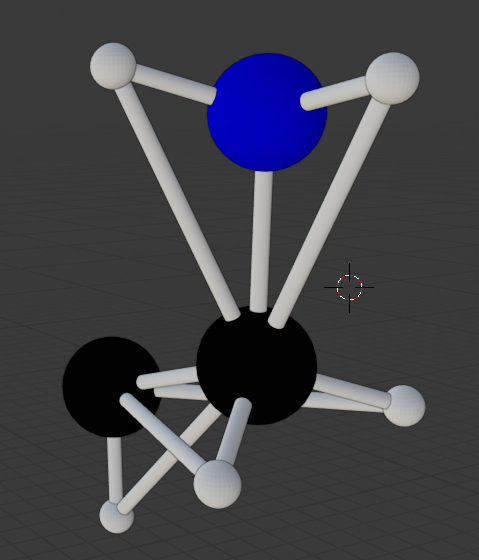
\includegraphics[width=\paperwidth/3]{bonds_wro.png}
&
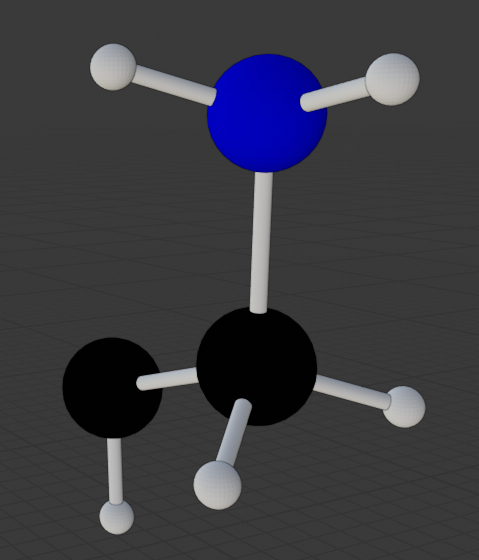
\includegraphics[width=\paperwidth/3]{bonds_cor.png}

\end{tabular}
\end{center}
\caption{Voorbeeld van kristal met foute bindingen (links) en correcte bindingen (rechts)}
\end{figure}
    

\subsection{CCTBX}
In de vierde sectie van hoofdstuk twee hebben de \textit{Computational Crystallography Toolbox} reeds besproken als een alternatief aan PyCIFRW om CIF-bestanden te parsen. Naast het parsen van bestanden heeft de cctbx nog een hele reeks aan andere functionaliteiten, waarvan veel erg handig kunnen zijn voor ons programma. Zo zou de cctbx niet enkel OpenBabel kunnen vervangen om de plaats van de atomen binnen de eenheidscel te berekenen, het is zelfs in staat de positie van alle atomen binnen bepaalde grenzen te berekenen, zoals we eerder in deze sectie hebben besproken.
\par
Het enige wat ons tegenhoudt cctbx te gebruiken is dat het erg moeilijk is deze werkende te krijgen op een Windowssysteem. In tegenstelling tot de installatie op Linux, welke met slechts één commando kan gedaan worden, is de installatie op Windows erg lastig. Zowel de installatiehandleiding die te vinden is op de website van cctbx, als de handleiding op hun GitHub pagina is gedateerd en voor dat de installatie kan worden uitgevoerd moeten er een aantal programma's geïnstalleerd zijn. We willen ook zeker zijn dat programma bruikbaar is op elk besturingssysteem en dat de installatie ervan niet te moeilijk is voor onervaren gebruikers. Dit alles heeft ertoe geleid dat er in dit onderzoek geen gebruik is gemaakt van de cctbx.

\section{conclusie}
In dit hoofdstuk zagen we eerst een stappenplan voor het gebruiken van onze add-on. Dit dient als handleiding die gebruikers kunnen volgen om de add-on te gebruiken zonder enige voorkennis nodig te hebben. 
\par
Uit de resultaten die we verkregen kunnen we concluderen dat de tekenduur van de add-on voor een klein kristal in de groteorde van enkele seconden zijn, terwijl dit voor grote kristallen naar enkele tientalle seconden neigt. De duur neemt ook toe wanneer we de tekenkwaliteit opdrijven. Het tekenen van bindingen zal aan deze tekenduur een vaste waarde toevoegen onafhankelijk van de tekenkwaliteit. Dit is omdat de kwaliteit enkel invloed heeft op de kwaliteit van de atomen en niet de bindingen.
\par    
In vergelijking met VESTA duurt het tekenen van een kristal beduidend langer bij onze add-on. Bij een klein kristal duurt het ongeveer 17 maal langer en deze factor neemt toe tot wel 400 bij een groot kristal. Deze langzaamheid is voornamelijk te wijten aan de bpy module welke eerder traag is. Door het uitvoeren van enkele testen hebben we waargenomen dat gemiddeld 80 procent van de loopduur van ons programma naar het tekenen van de atomen gaat. 
\par
Op het vlak van gebruiksvriendelijk heeft onze add-on enkele verschillen ten opzichte van VESTA, zo heeft onze add-on minder features, maar is het eenvoudiger in gebruik en is het kristalmodel interactiever dan dat van VESTA. Welk programma nu juist het meest geschikt is op vlak van gebruiksvriendelijk hangt voornamelijk van de toepassing af. Een groot voordeel dat onze add-on heeft over VESTA is dat het enorm eenvoudig uit te breiden is, terwijl een gebruiker VESTA moeilijk of zelfs niet kan uitbreiden. Dit maakt de add-on erg "future proof".
\par 
Een probleem waar we in dit onderzoek mee hebben gekampt is het moeilijk vinden van online informatie over de nieuwste versie van de Blender API, die we gebruiken in onze add-on. Doordat de verschillen tussen Blender 2.80 en oudere versies van Blender zijn veel technieken die vroeger mogelijk waren niet meer van toepassing en zijn er weinig voorbeelden van toepassingen die wel werken. Door de goede documentatie van de Blender API was dit echter geen enorm probleem.
\par
Door een probleem met de CifFile module is het tot heden niet mogelijk bestanden met lange padnamen in te lezen. Hierdoor kan onze add-on niet functioneren zonder dat de gebruiker OpenBabel heeft geïnstalleerd. Dit probleem kan voorlopig niet worden opgelost. 
\par
We hebben enkele features gezien die mogelijks kunnen worden toegevoegd aan de add-on. Door de gebruiker zelf grenzen te laten kiezen waartussen het kristal moet worden getekend kan deze zelf de grootte van het kristal bepalen, voorlopig worden enkel de atomen binnen de eenheidscel getekend.
\par
Door een dictionary toe te voegen die de bindingsafstand per atoom bevat, hoeft de gebruiker niet meer manueel de bindingsafstand te bepalen. Dit zal leiden tot minder foute bindingen.
\par
Ten slotte hebben we geleerd dat de cctbx een krachtige tool is met erg veel functiess die onze add-on kunnen worden gebruikt. Op dit moment wordt er in onze add-on nog geen gebruik gemaakt van de cctbx, dit komt doordat deze erg moeilijk te installeren is op een Windowssysteem.  


 
   